\documentclass[11pt, oneside]{article} 
\usepackage{geometry}
\geometry{letterpaper} 
\usepackage{graphicx}
	
\usepackage{amssymb}
\usepackage{amsmath}
\usepackage{parskip}
\usepackage{color}
\usepackage{hyperref}

\graphicspath{{/Users/telliott/Github/number_theory/png/}}
% \begin{center} \includegraphics [scale=0.4] {gauss3.png} \end{center}

\title{Euler's totient}
\date{}

\begin{document}
\maketitle
\Large

Euler's totient function is symbolized by $\phi(n)$.

$\phi$ gives a count of how many numbers in the set $ \{ 1, 2, 3 \dots , n-1 \}$, that is, $a \in \mathbb{N} \ | \ a < n$

share no common factors with $n$ other than $1$, i.e. that have a gcd with $n$ equal to $1$.  We include $1$ in the count.

If $n$ is prime, this is easy.  

For a prime $p$, the only number that evenly divides $p$ is $1$ (and $1$ always has a gcd of $1$ with another integer), so the count of numbers less than $p$ that have gcd $= 1$ is $p - 1$.

\subsection*{non-primes}

Otherwise, it gets more difficult.  

The fundamental theorem of arithmetic says that any number $n$ has a \emph{unique} prime factorization.

There is another theorem that says that if we have the prime factors of $n$:
\[ n = p_1 \cdot p_2 \cdot p_3 \dots \]
    
then

\[ \phi(n) = \phi(p_1) \cdot \phi(p_2) \cdot \phi(p_3) \dots \]

This is true not just for primes, but for any two coprime factors of $n$.  

This will explain why we are able to write (in deriving an RSA key), that since $n = p \cdot q$:
\[ \phi(n) = (p-1)(q-1) \]

So if
\[ \phi(n) = \phi(p_1) \ \phi(p_2) \ \phi(p_3) \dots \]
    
We can multiply and divide by the product of the prime factors of $n$ and obtain

\[ \phi(n) = \frac{p_1 \ p_2 \dots}{p_1 \ p_2 \dots} (p_1 - 1) \ (p_2 - 1) \ \dots \]
\[ \phi(n) = n(p_1 - 1/p_1)(p_2 - 1/p_2) \ \dots \]

I found a nice write-up of this here:

\url{http://www.claysturner.com/dsp/totient.pdf}

In the write-up there is a sketch of a proof of the last line above, and you can follow it backward to what we were given:
\[ \phi(n) = \phi(p_1) \cdot \phi(p_2) \cdot \phi(p_3) \dots \]

\subsection*{example}
Consider $n = 30$.  If we run Euclid's algorithm on $1 < m < n$, we can find numbers that are coprime to (do not share any factor with) $30$:

\begin{verbatim}
 7 11 13 17 19 23 29
\end{verbatim}

These are the primes smaller than $n$, excluding those that divide $n$.

The set we seek includes $1$, hence $\{ 1, 7, 11, 13, 17, 19, 23, 29 \}$.

These are the numbers that are not included in the Venn circles:

\begin{center} 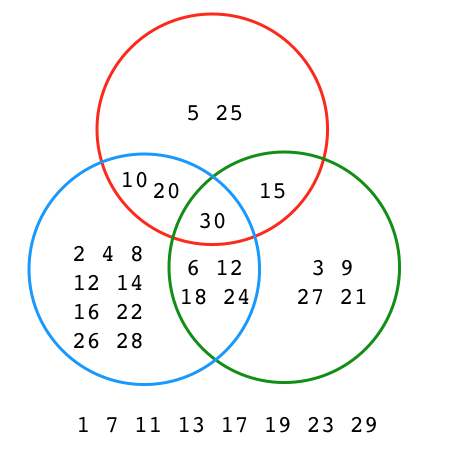
\includegraphics [scale=0.4] {/fermat-30.png} \end{center}

The prime factors of $30$ are $2$, $3$ and $5$.  

We can divide $1 \le m \le n$ into several sets:

$\circ$ \ $n$ itself

$\circ$ \ prime factors of $n$:  $2$, $3$ or $5$

plus

$\circ$ \ gcd equal to a single prime factor

$\circ$ \ gcd equal to a product of prime factors

and last

$\circ$ \ 1

$\circ$ \  prime, not a factor of $n$

We are trying to count the last group.

Let

$\circ$ \ $A$ be the set of integers that $2$ divides into evenly, including $n$

$\circ$ \ $B$ be the set .. $3$

$\circ$ \ $C$ be the set .. $5$

We want to find the count or size of the set of all the numbers that are not in A, B or C (the numbers listed along the bottom of the figure).

This is sizeof $\neg (A \cup B \cup C)$
    
where $\neg$ symbolizes the complement of the set, those elements not in the given set, and $\cup$ is set union.

There is a famous theorem in set theory that says: 
\[ \neg(A \cup B \cup C) = (\neg A) \cap (\neg B)  \cap (\neg C) \]

$ \cap$ is set intersection.

so we want the size of the right-hand side.

\subsection*{using probability}

It is somewhat surprising, but we can easily calculate the probability that a number is in the set $\neg A$.  

Consider the set including $2$ and all its multiples.  The probability that a number $\le 30$ is contained in the complement of that set is $1 - 1/2$, the fraction of all numbers that are even, times $30$.  

Similarly, for $~B$, the probability is $1 - 1/3$ times $30$ and so on.

The total probability is the product of the individual probabilities.

And that total probability, times $n$, is equal to the count.

Thus
\[ \phi(30) = \ \text{sizeof} \  (\neg A) \cap (\neg B)  \cap (\neg C) \]
\[  = 30 \cdot (1 - 1/2) \cdot (1 - 1/3) \cdot (1 - 1/5) \]
    
And generalizing

\[ \phi(n) = n \cdot (1 - 1/p_1) \cdot (1 - 1/p_2) \dots \]
    
which is what we needed to prove.

$\square$

This can be rewritten as
\[ \phi(n) = (p_1 - 1) \cdot (p_2 - 1) \dots \]

\subsection*{goal}

For cryptography, what we're looking for is a function that has an inverse, where
\[ (m^e)^d = (m^d)^e = m \]
Always, mod $n$.

So with Euler's extension of Fermat's little theorem (substituting $m$ for $a$):
\[ m^{\phi(n)} = 1 \]
    
In this case, raising to the power $k$ doesn't change the result:
\[ m^{k \cdot \phi(n)} = 1\]
\[ m^{k \cdot \phi(n) + 1} = m \]

So, we see that it will work to find
\[ e \cdot d := k \cdot \phi(n) + 1 \]

And thus
\[ e \cdot d := 1 \ mod \ \phi(n) \]

And that's why it works.


\end{document}